\section{Ranking of structural Ricardian comparative advantage }
In this section I present the results of the structural RCA ranking for both value-added exports measures and gross exports. First, I will take a global view and analyze the results of the association by plotting the coefficients against a country's per capita GDP. The hypothesis is that country's with a higher GDP show a higher similarity between the rankings and that for poorer countries the sourcing and factor usage is more sector specific. \par Second, I will view at the structural RCA results by comparing the rankings for Belgium and Germany of forward and backward value-added exports to gross exports. In this way, I analyze whether there different perspectives of value-added exports affect the comparative advantage ranking. 
\subsection{Structural Ricardian comparative advantage based gross exports and value-added exports}
\begin{figure}
\caption{Association RCA based on VAX \& EXGR and GDP per capita }
\centering
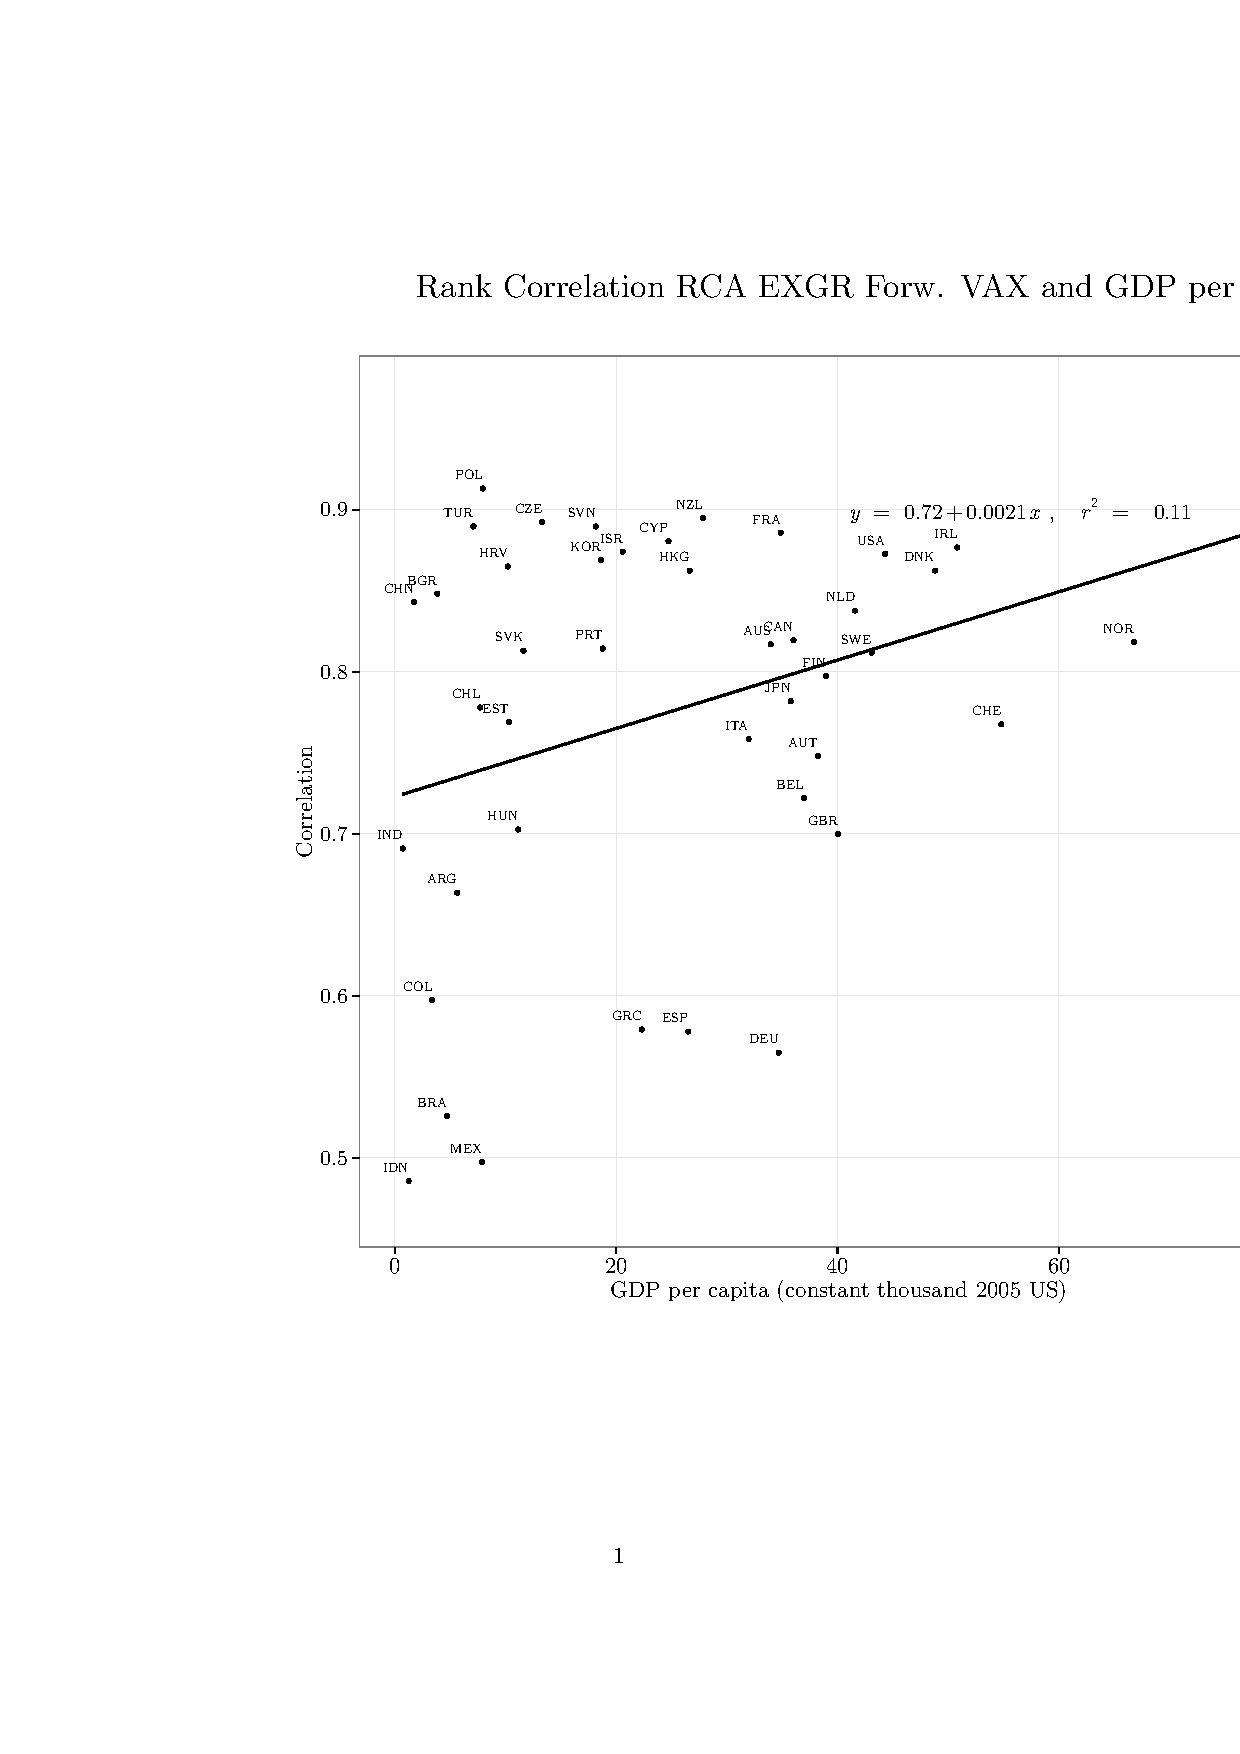
\includegraphics[width=.49 \linewidth]{./fig/spearman_fddva_std_balassa-march.tex}
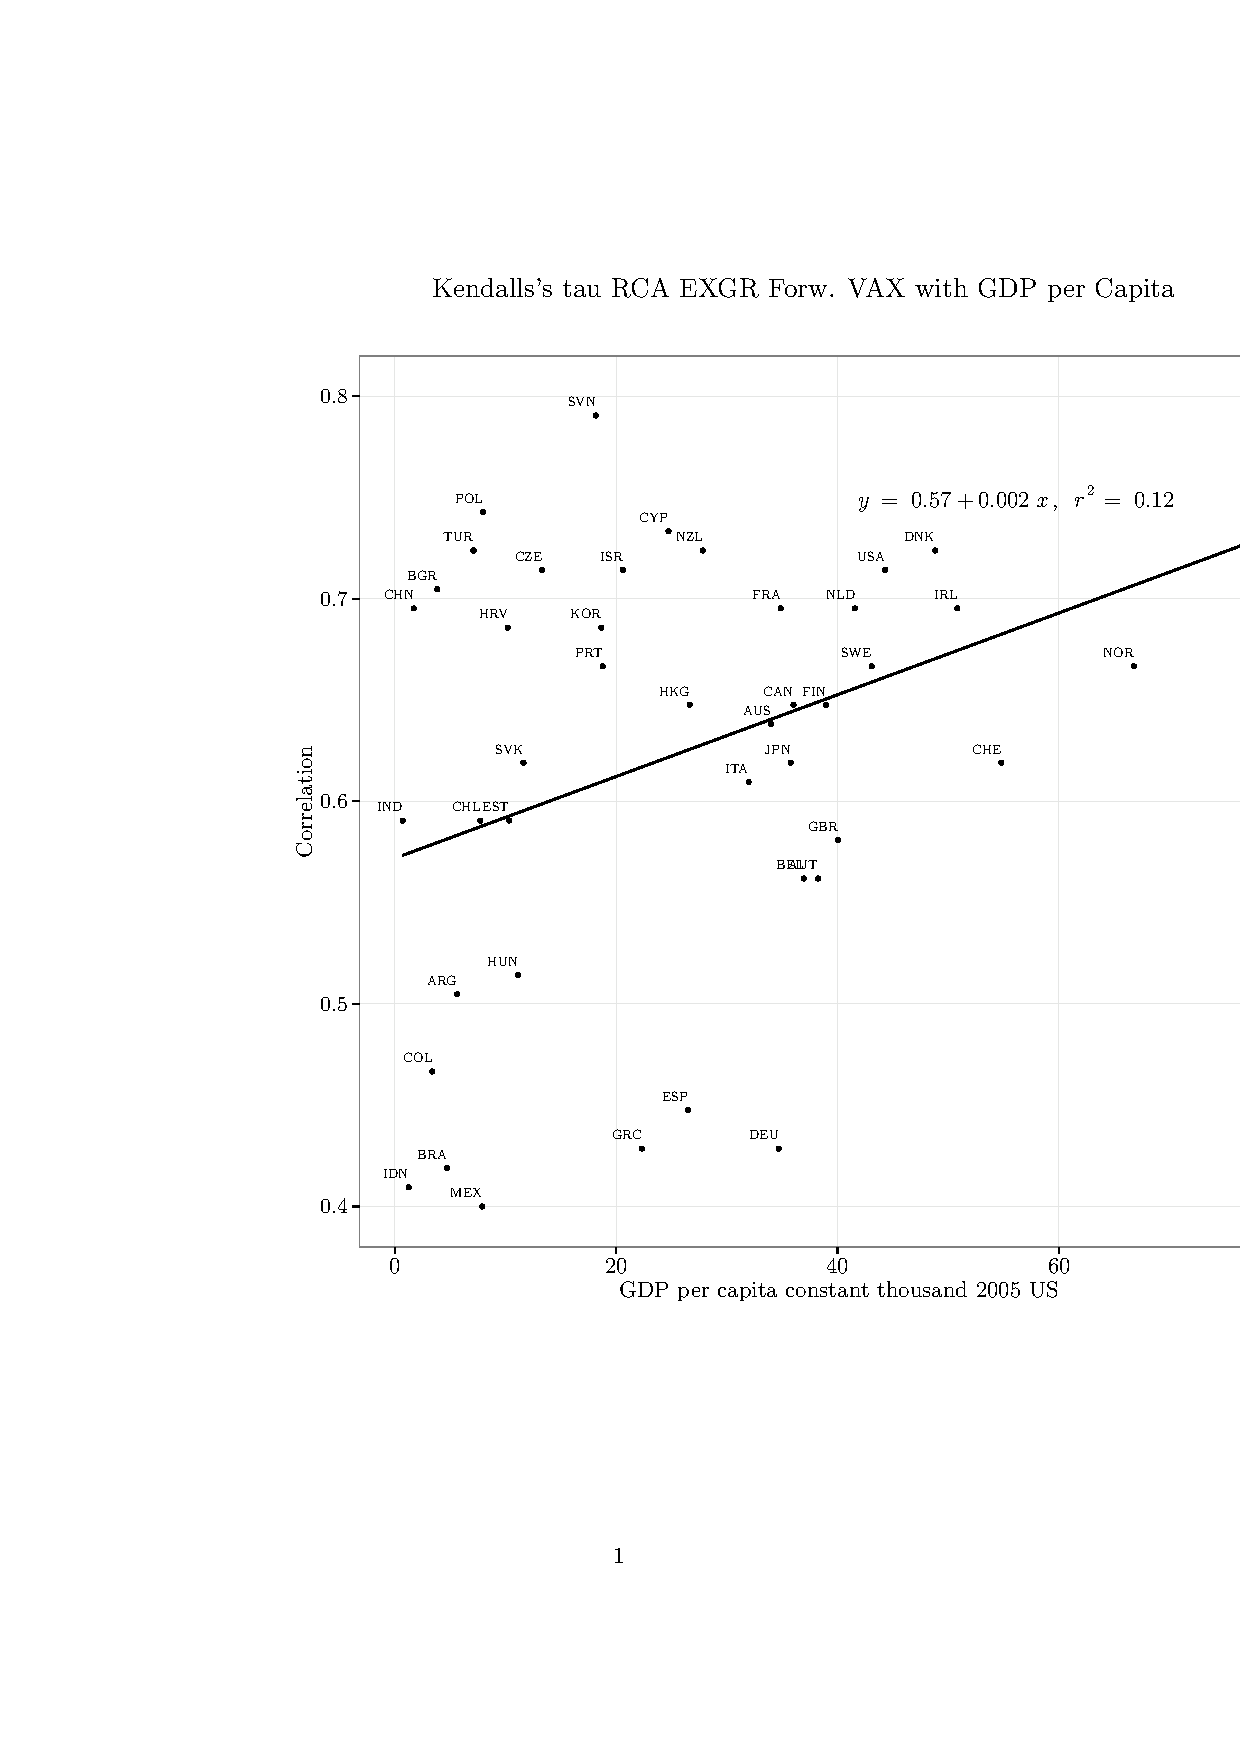
\includegraphics[width=.49 \linewidth]{./fig/kendall_fddva_exgr_std_balassa-march.tex}
 %\captionof{figure}{Another figure}
\end{figure}
\begin{figure}
\caption{Country pair RCA based on for- and backward  VAX \& EXGR }
\includegraphics[width=.5\linewidth]{./fig/back_exgr_DEU_BEL_tiva.tex}
\includegraphics[width=.5\linewidth]{./fig/forw_exgr_DEU_BEL_tiva.tex}
\end{figure}

\endinput